\textcolor{Black}{
In the following section the system is modeled with Alloy\cite{alloy} to check that the contracts' execution flow is correct and
that related actions such as opening a discussion or giving a feedback can be performed only in the intended phases.
}
\begin{minted}[breaklines]{alloy}
// Signatures
sig User {
	name: one String
}

sig Student extends User {
	university: one University,
	skills: set String
}

sig Company extends User {
	internships: set Internship
}

sig University extends User {}

sig Internship {
	offeredBy: one Company,
	title: one String,
	skillsRequired: set String
} { this in offeredBy.internships }

sig Contract {
	internship: one Internship,
	student: one Student,
	var status: one ContractStatus
}

enum ContractStatus { Pending, Accepted, OnGoing, Rejected, Expired, Interrupted }

sig Discussion {
	owner: one User,
	contract: one Contract,
	messages: set DiscussionMessage
} { (owner not in University) and 
	(owner = contract.student or owner = contract.student.university or owner = contract.internship.offeredBy) and
	(all m: DiscussionMessage | m in messages implies (m.sender = contract.student or m.sender = contract.student.university or m.sender = contract.internship.offeredBy))}

sig DiscussionMessage {
	sender: one User,
	content: one String
} { one d: Discussion | this in d.messages }

sig Feedback {
	contract: one Contract,
	author: one User,
	content: one String,
	rating: one Int
} { author in contract.student + contract.internship.offeredBy and rating >= 1 and rating <= 5}

// Flow control
fact newIsPending {
	all c: Contract | c.status = Pending
}

// Possible flows
pred NormalFlow[c: Contract] { (c.status = Pending ; c.status = Accepted ; c.status = OnGoing ; always c.status = Expired) }
pred InterruptedFlow[c: Contract] { (c.status = Pending ; c.status = Accepted ; c.status = OnGoing ; always c.status = Interrupted) }
pred RejectedFlow[c: Contract] { (c.status = Pending ; always c.status = Rejected) }

// No other flows other that the ones listed
fact NoOtherFlows { 
	no c: Contract | 
		not c.RejectedFlow and
		not c.InterruptedFlow and
		not c.NormalFlow
}

// General facts

// Every User is a Student, Company or Univesity
fact AllUsersSubclassed { all u: User | u in Student + Company + University }

// Each Student can't apply twice to the same internship
fact CannotApplyTwiceToAnInternship {
	all c1, c2: Contract | (c1.student = c2.student and c1.internship = c2.internship) implies c1 = c2
}

// To interrupt a contract, a discussion must have been opened at least once
fact InterruptionNeedDiscussion {
    always (all c: Contract | c.status = Interrupted implies (some d: Discussion | d.contract = c))
}

// Can't give feedback if the contract has reached an end (the contract must have not been rejected)
fact FeedbackAllowedOnlyIfCompletion {
    always (all f: Feedback, c: Contract | c = f.contract implies eventually c.status in (Expired + Interrupted))
}

// Can't Open a discussion if the contract has been rejected
fact NoDiscussionIfRejectcion {
	 always (all d: Discussion, c: Contract | c = d.contract implies c.status not in Rejected)
}

// Can't give multiple feedbacks to the same internship experience
fact NoMultipleFeedbacks{
    all f1, f2: Feedback |
        (f1.contract = f2.contract and f1.author = f2.author) implies f1 = f2
}

// Every internship is posted by a company
fact EveryInternshipHasACompany {
    all i: Internship | one c: Company | i in c.internships
}

// No multiple students working in the same internship at the same time
fact NoMultipleOngoingContractForSameIntership {
    always all c1,c2: Contract | (c1.status = OnGoing and c2.status = OnGoing and c1.internship = c2.internship) implies c1.student = c2.student
}

// To match students and companies there must be at least one matching skill between them
fact MatchingSkillsDuringContractCreation {
    all c: Contract |
        some c.student.skills & c.internship.skillsRequired
}

// Assertions

// Duplicate applications for the same combination of student and internship are not allowed
assert NoDuplicateApplications {
    all c1, c2: Contract |
        (c1.student = c2.student and c1.internship = c2.internship) implies c1 = c2
}

check NoDuplicateApplications for 10

// DiscussionMessages can be sent only by the parties of the Contract or the University of the contracted Student
assert NoMessagesFromSenderOutsideContract{
    all d: Discussion, m: DiscussionMessage, c: Contract | 
	(d.contract = c and m in d.messages) implies 
		((d.owner = c.student or d.owner = c.internship.offeredBy) and
		(m.sender = c.student or m.sender = c.student.university or m.sender = c.internship.offeredBy))
}

check NoMessagesFromSenderOutsideContract for 10

// Show
// Show with matching skills
pred ShowWithSkills {
    some u: University, s: Student, c: Company, i: Internship {
	   (some con: Contract | con.NormalFlow)
        s.university = u
        s.name = "Pluto"
        s.skills = "java" + "c"
        i.skillsRequired = "java" + "python"
        i in c.internships
	   i.title = "Programmer"
	   u.name = "Polimi"
	   c.name = "PoliGrammer"
    }
}

// Show normal flow of action
pred ShowSingle {
	some u: University, s: Student, c: Company, i: Internship {
	(some con: Contract | con.NormalFlow)
		s.university = u
        	s.name = "Pluto"
       	i in c.internships
    }
}

// Show interrupted contract
pred ShowInterrupted {
	some u: University, s: Student, c: Company, i: Internship {
	(some con: Contract | con.InterruptedFlow)
		s.university = u
        	s.name = "Pluto"
       	i in c.internships
    }
}

// General show (no required skills)
pred Show {
	some u: University, s: Student, c: Company, i: Internship {
		(some con: Contract | con.RejectedFlow)
		(some con: Contract | con.NormalFlow)
		(some con: Contract | con.InterruptedFlow)
        	s.university = u
	  	s.name = "Pluto"
       	i in c.internships
    }
}

// Single
run ShowSingle for 4 but exactly 1 Contract, exactly 1 Student,exactly 1 Company, exactly 1 University, exactly 1 Internship

// Status progression
run Show for 4 but exactly 3 Contract, exactly 2 Student, 3 Company, 2 University, 4 Internship, exactly 1 Discussion, exactly 0 Feedback

// Feedback
run Show for 4 but exactly 1 Student, exactly 1 Company, 1 University, exactly 4 Feedback

// Discussion
run ShowInterrupted for 4 but exactly 1 Contract, exactly 1 Student, exactly 1 Company, exactly 1 University, exactly 1 Internship, exactly 2 Discussion, exactly 3 DiscussionMessage

// Skill matching
run ShowWithSkills for 4 but exactly 1 Contract, exactly 1 Student,exactly 1 Company, exactly 1 University, exactly 1 Internship, exactly 0 Feedback, exactly 0 Discussion
\end{minted}
\newpage
\subsection{Examples}
\textcolor{Black}{
An example of a contract's standard progression where it eventually expires without any issues.\\
}
\mintinline[breaklines]{alloy}{run ShowSingle for 4 but exactly 1 Contract, exactly 1 Student,exactly 1 Company, exactly 1 University, exactly 1 Internship}\\
\begin{figure}[h]
    \centering
    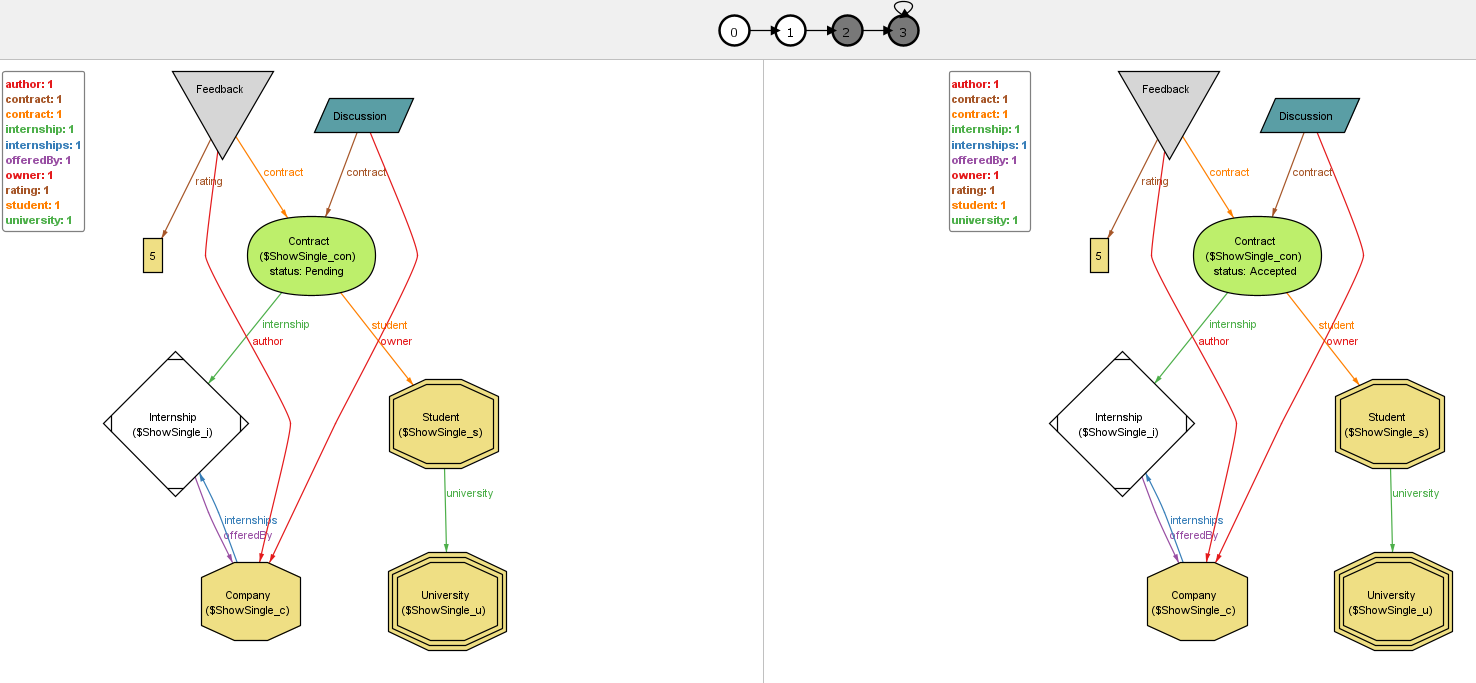
\includegraphics[width=1\linewidth]{Images//Alloy/1.png}
    \caption{ShowSingle, first two steps}
\end{figure}
\begin{figure}[h]
    \centering
    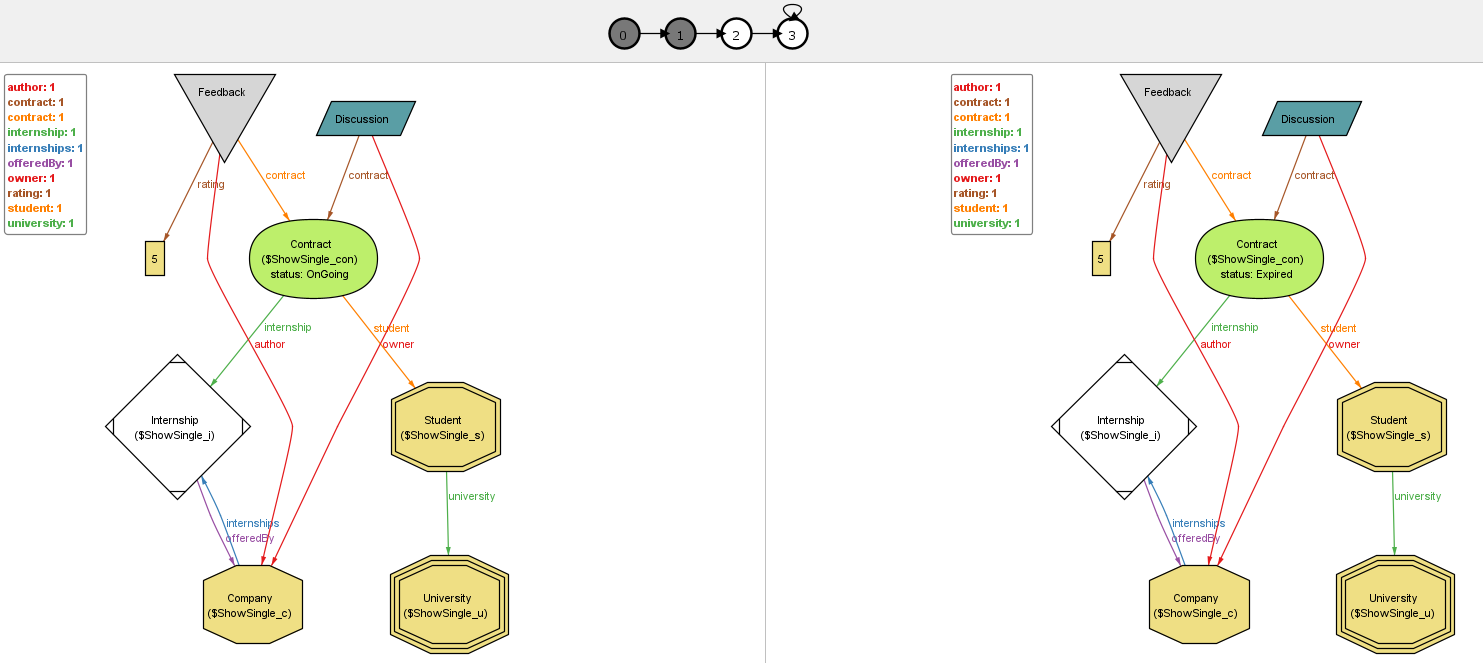
\includegraphics[width=1\linewidth]{Images//Alloy/2.png}
    \caption{ShowSingle, first two steps}
\end{figure}
\newpage
\textcolor{Black}{
An example of the progression for every contract.\\
}
\mintinline[breaklines]{alloy}{run Show for 4 but exactly 3 Contract, exactly 2 Student, 3 Company, 2 University, 4 Internship, exactly 1 Discussion, exactly 0 Feedback}
\begin{figure}[h]
    \centering
    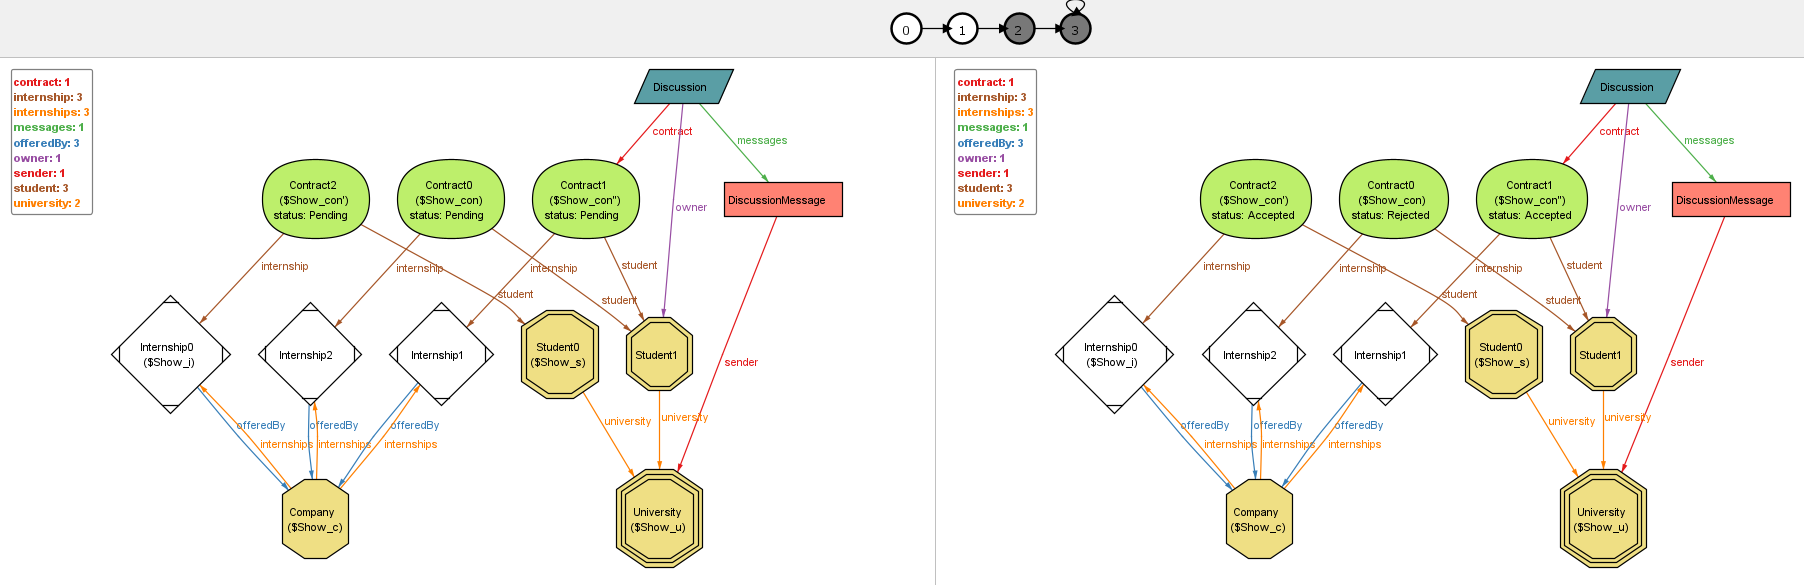
\includegraphics[width=1\linewidth]{Images//Alloy/3.png}
    \caption{Show, first two steps}
\end{figure}
\begin{figure}[h]
    \centering
    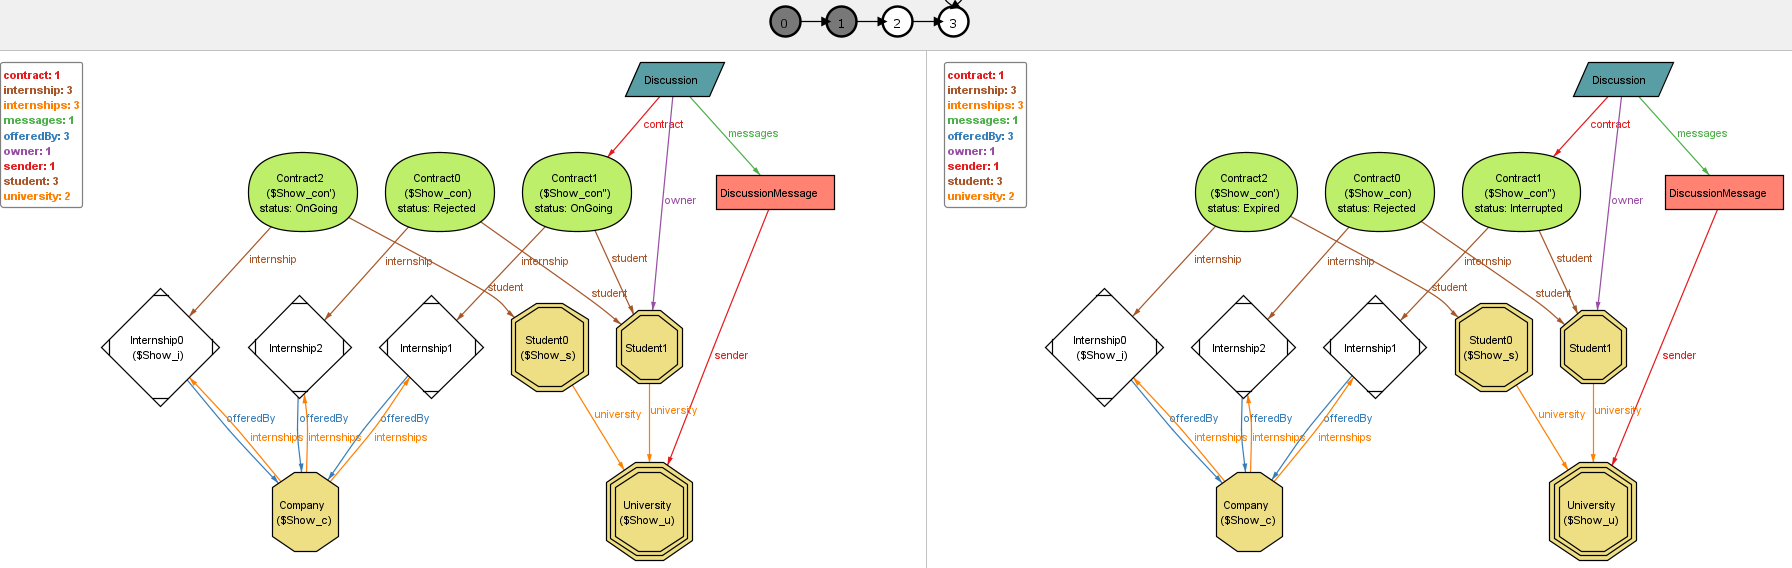
\includegraphics[width=1\linewidth]{Images//Alloy/4.png}
    \caption{Show, last two steps}
\end{figure}
\newpage
\textcolor{Black}{
An example showing that every non-rejected contract can have feedback from both parties involved in the contract.\\
}
\mintinline[breaklines]{alloy}{run Show for 4 but exactly 1 Student, exactly 1 Company, 1 University, exactly 4 Feedback}
\begin{figure}[h]
    \centering
    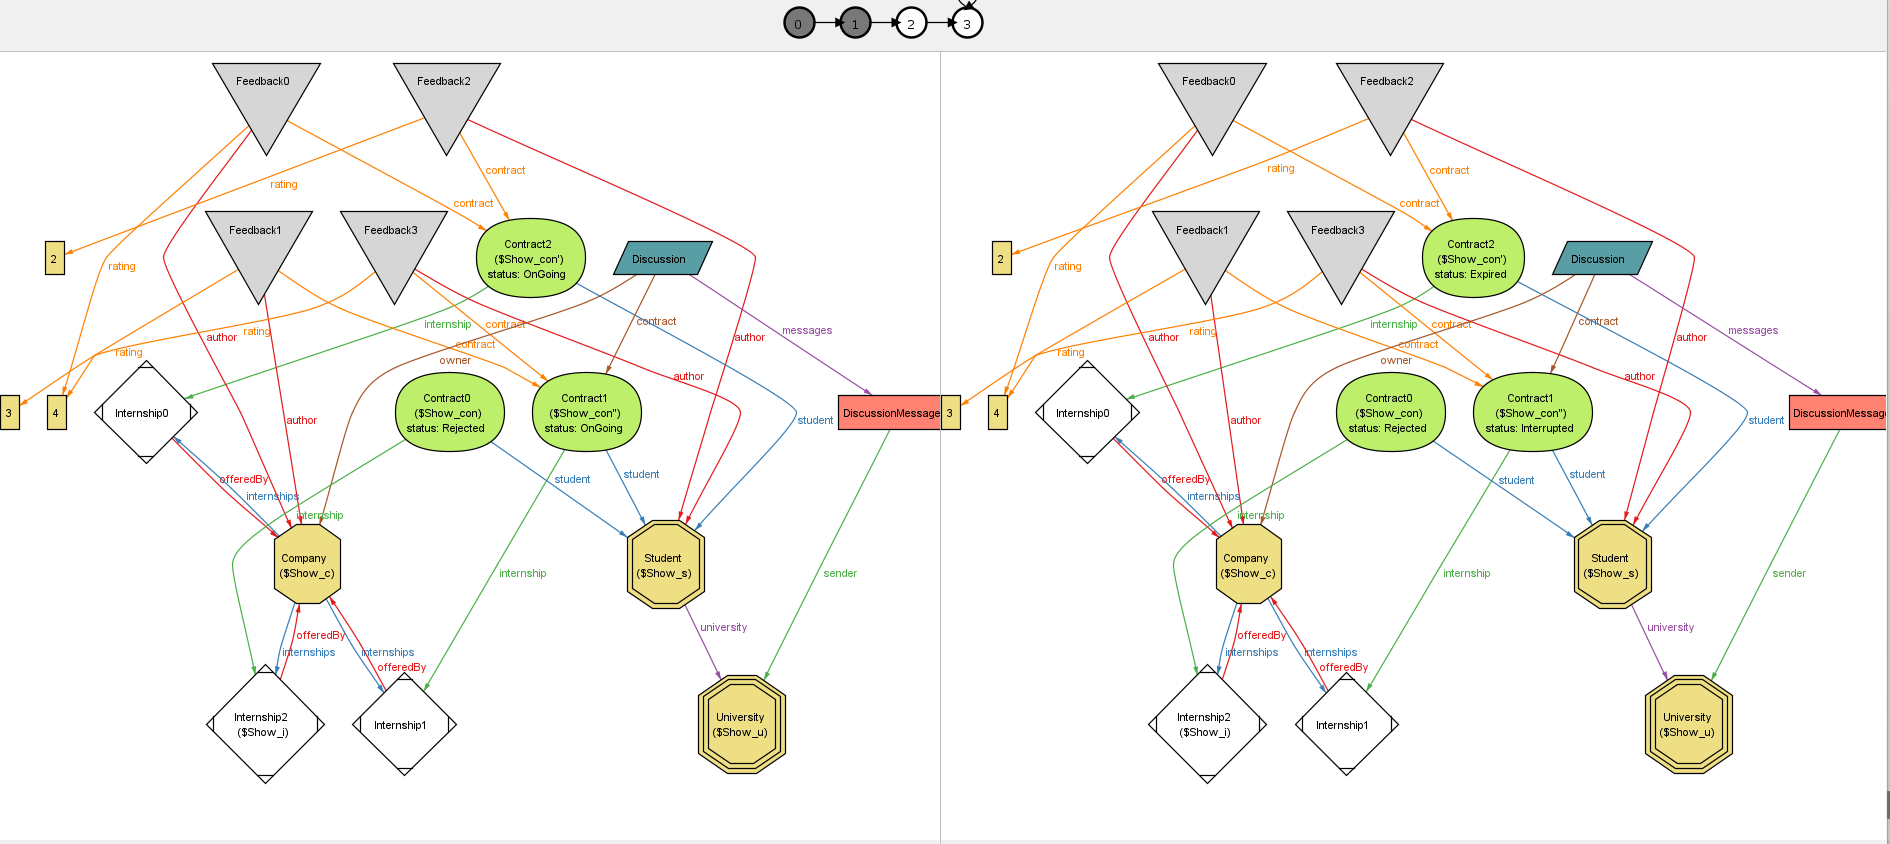
\includegraphics[width=1\linewidth]{Images//Alloy/5.png}
    \caption{Show with Feedback, last two steps}
\end{figure}
\\
\textcolor{Black}{
An example demonstrating how the interruption of a contract works (at least one discussion must have been created beforehand).\\
}
\mintinline[breaklines]{alloy}{run ShowInterrupted for 4 but exactly 1 Contract, exactly 1 Student, exactly 1 Company, exactly 1 University, exactly 1 Internship, exactly 2 Discussion, exactly 3 DiscussionMessage}
\begin{figure}[h]
    \centering
    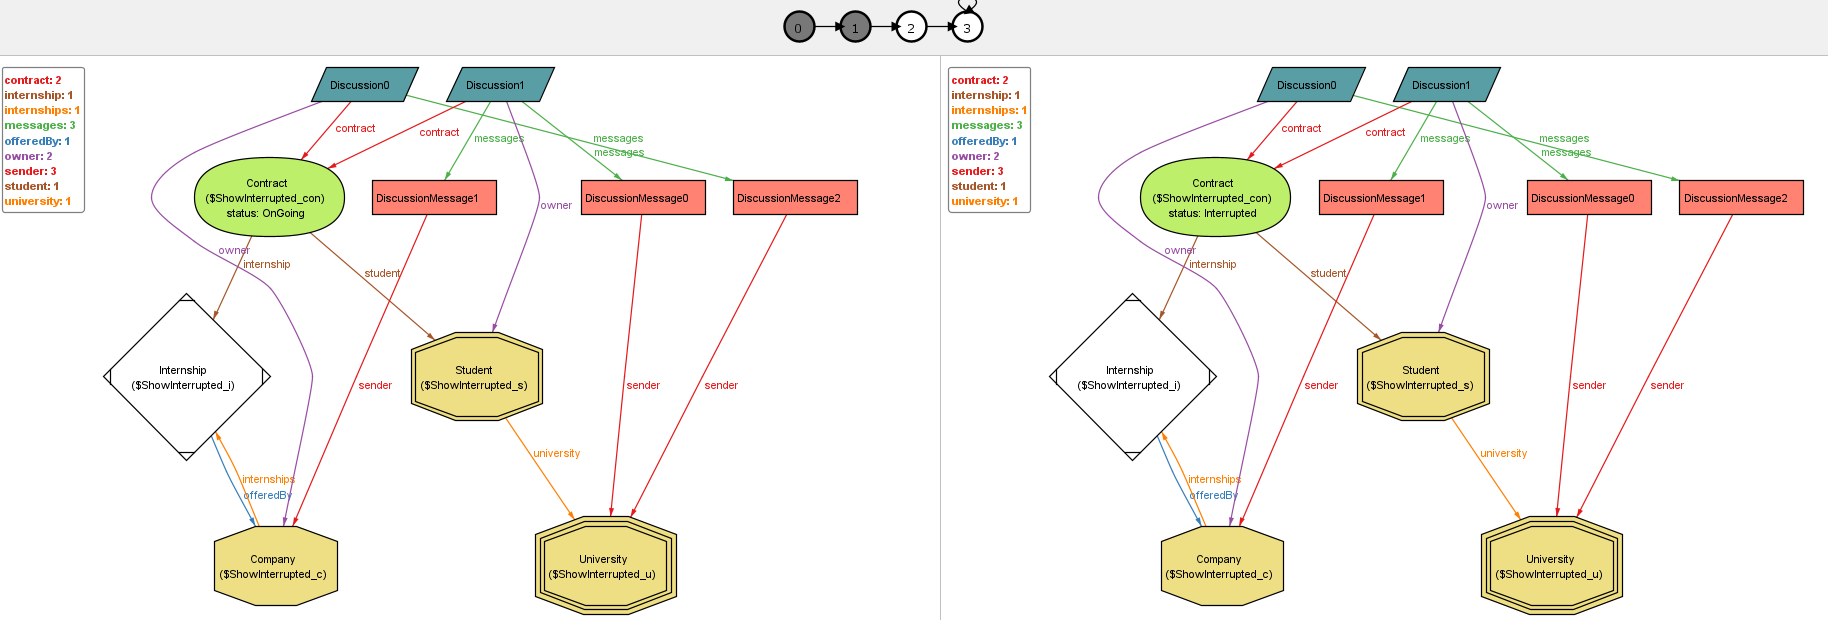
\includegraphics[width=1\linewidth]{Images//Alloy/6.png}
    \caption{ShowInterrupted, last two steps}
\end{figure}
\newpage
\textcolor{Black}{
An example illustrating how skill matching works.\\
}
\mintinline[breaklines]{alloy}{run ShowWithSkills for 4 but exactly 1 Contract, exactly 1 Student,exactly 1 Company, exactly 1 University, exactly 1 Internship, exactly 0 Feedback, exactly 0 Discussion}
\begin{figure}[h]
    \centering
    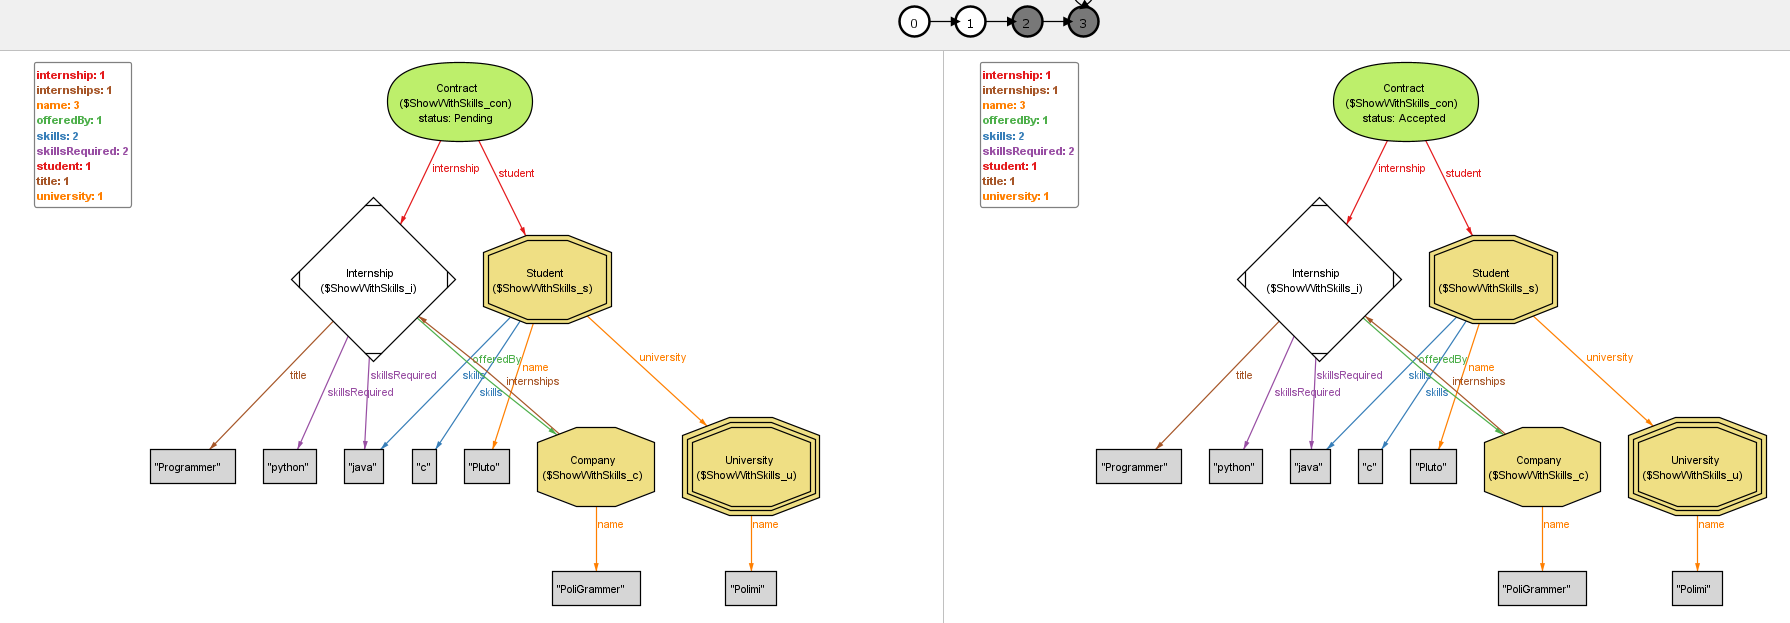
\includegraphics[width=1\linewidth]{Images//Alloy/7.png}
    \caption{ShowWithSkills, first two steps}
\end{figure}

\textcolor{Black}{
\paragraph{Checks\\}
Every check terminated without finding counterexamples, showing that the checked are valid.
}